\documentclass[11pt, a4paper]{article}

\usepackage[margin=1in]{geometry} % Set margins.
\usepackage{enumitem} % Customize lists.
\usepackage{hyperref} % For hyperlinks.
\usepackage{titlesec} % Custom section titles.
\usepackage{graphicx} % Required for including images
\usepackage{float} % For precise placement of the figure
\usepackage{fontawesome} % For icons
\usepackage{adjustbox}
\usepackage{tikz}


% Set section title formatting
\titleformat{\section}
{\large\bfseries} % Format
{} % Label
{0em} % Sep
{} % Before-code
[\titlerule] % After-code

\pagestyle{empty} % No page numbers

\begin{document}
\noindent
\begin{minipage}{0.25\textwidth}
    \begin{tikzpicture}
        % Define variables
        \def\xCenter{-0.1} % X center of the circle
        \def\yCenter{0.65} % Y center of the circle
        \def\circleRadius{1.9} % Radius of the circle
        
        % Clipping for the image
        \clip (\xCenter,\yCenter) circle (\circleRadius cm);
        
        % Place the image
        \node at (0, 0) {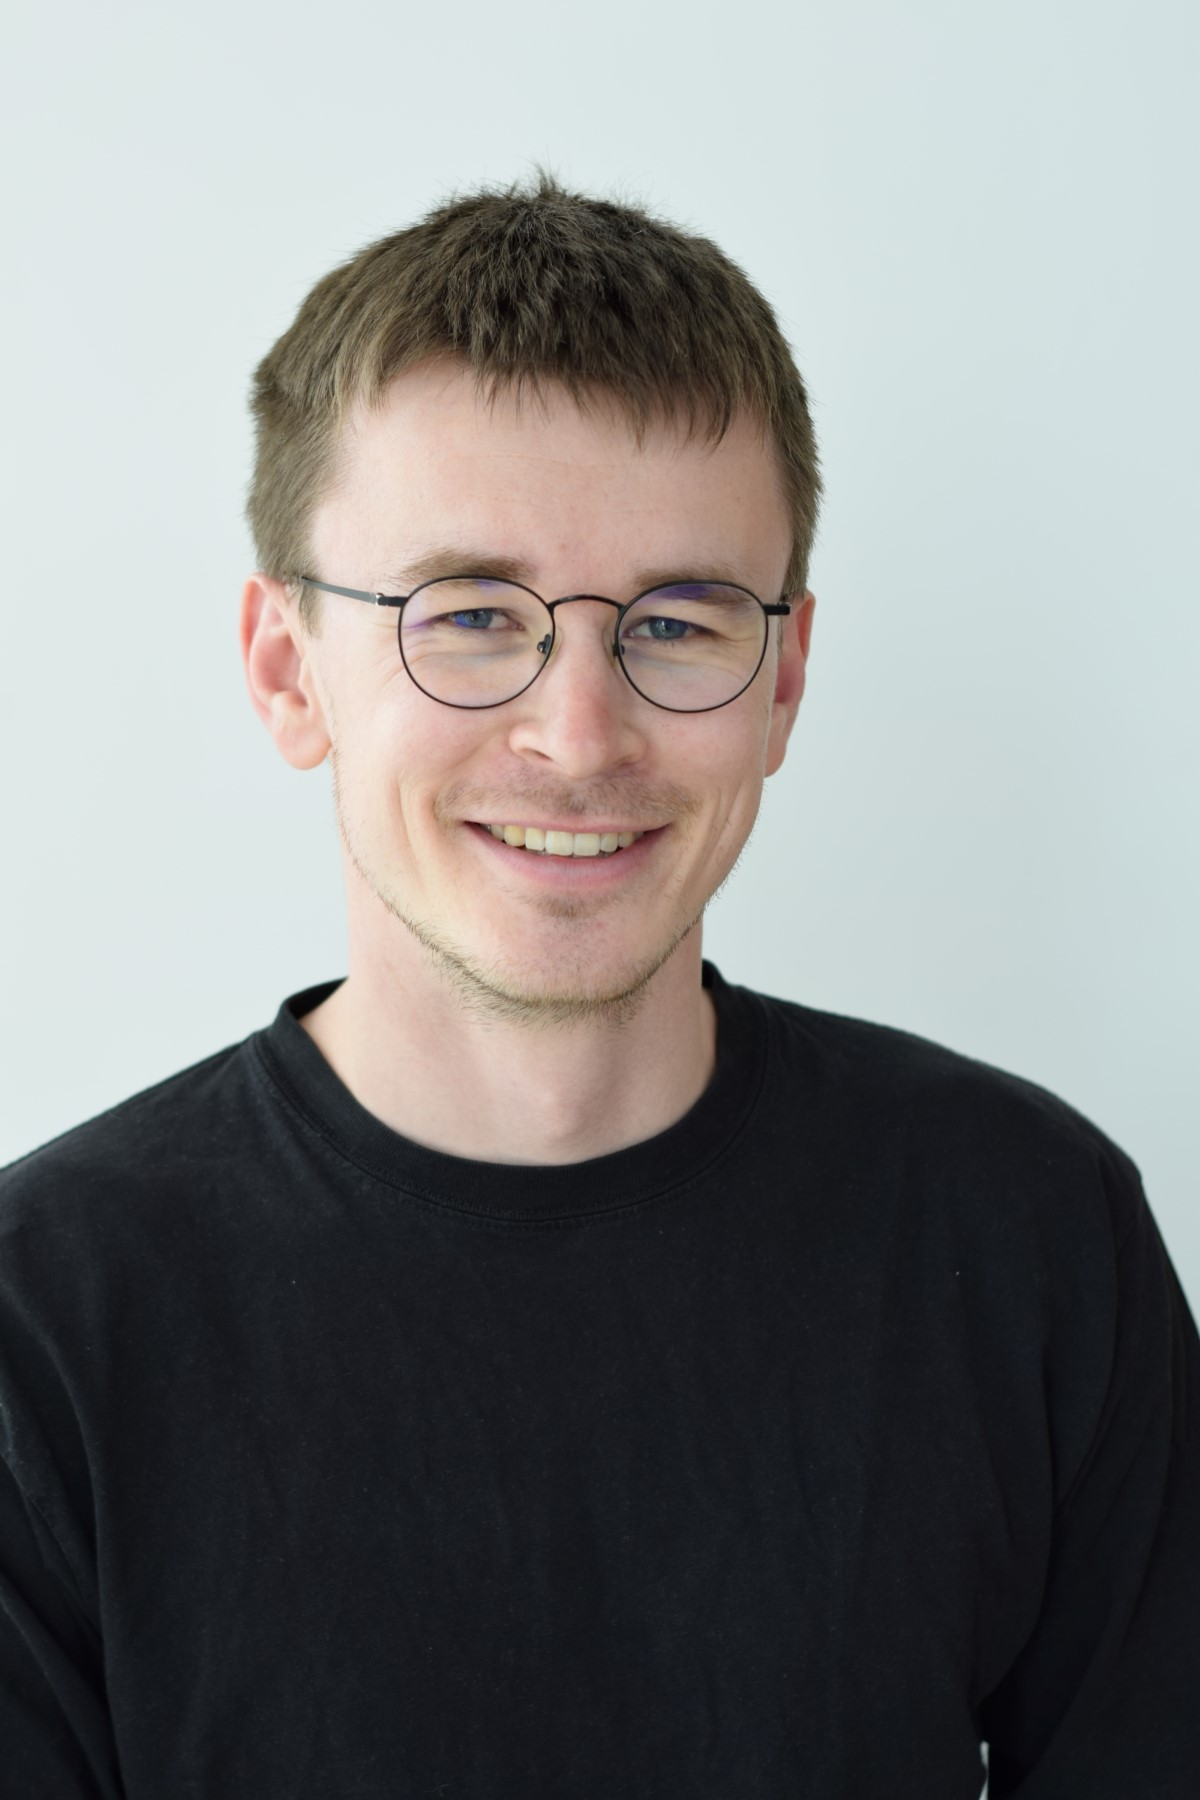
\includegraphics[height=6cm]{./assets/profile_pic_small.jpg}};
        
        % Draw the circular border
        \draw[gray, thick] (\xCenter,\yCenter) circle (\circleRadius cm); % Adjust 'thick' as needed for border width
    \end{tikzpicture}

\end{minipage}%
\begin{minipage}{0.75\textwidth}
    \centerline{
        \Large\bfseries Frej Sundqvist
    }
    \vspace{0.2em}
    \centerline{
        \textit{Problem solver, Programmer, Engineer}
    }
    \centerline{
        From Sweden, living in Norway
    }
    \vspace{0.5em}
    \centerline{
        {\faEnvelopeO} \href{mailto:frejsundqvist@protonmail.com}{frejsundqvist@protonmail.com}
        |
        {\faGithub} \href{https://github.com/MyosQ}{MyosQ}
    }
    \centerline{
        {\faLinkedin} \href{https://linkedin.com/in/frej-sundqvist-b8a49a14b}{frej-sundqvist-b8a49a14b}
        |
        {\faGlobe} \href{https://myosq.github.io/cv}{myosq.github.io/cv}    
    }
\end{minipage}

\vspace{1em}

\section*{Experience}
\textbf{Fullstack Engineer, Tech lead}, \textit{Capia AS}, Tromsø, Norway \hfill 2021 - Present
\begin{itemize}[noitemsep]
    \item Building webapps in django/django$+$react from scratch to deployment.
    \item Building and managing 10$+$ CI/CD pipelines for different projects using Github Actions and Bitbucket Pipelines.
    \item Leading teams of 3$+$ developers and interacting directly with customers.
    \item Fine-tuning Neural Networks for image segmentation and classification.
    \item Linux system administering - Managing Nginx, backup procedures, and server security.
\end{itemize}

\section*{Education}
\textbf{Master's degree in Engineering Physics}\\
\textit{Specialization: Computational Physics}

\begin{itemize}[noitemsep]
    \item Umeå university, Sweden \hfill 2015 - 2021
    \item Julius-Maximilians-Universität, Würzburg, Germany \hfill 2018 - 2019
\end{itemize}

\section*{Skills}
\begin{itemize}[noitemsep]
    \item Python, C, JavaScript, Rust, R, Matlab, PHP, 
    \item Django, Pytorch, Pandas, Numpy,
    \item Git, Docker, Docker-compose, Kubernetes, Github/Gitlab/Bitbucket CI/CD,
    \item SQL, NoSQL, MariaDB, PostgreSQL, PostGis, Redis,
    \item Google Cloud, Cloudflare, Backblaze,
    \item Apache Airflow, Kafka,
    \item React, Nodejs, HTML, CSS, LESS, 
    \item Linux System Administration, Network protocols, Bash, Nginx,
\end{itemize}

\section*{Other work}
\textbf{Math's Solution Expert}, \textit{\href{https://logio.se}{Logio}} Stockholm \hfill 2017 \\
    Part-time work delivering pedagogical solution to math problems in the Swedish
    ”Högskoleprovet”.


\section*{Languages}
\begin{itemize}[noitemsep]
    \item Swedish: Native
    \item English: Fluent
    \item German: Fluent
    \item Norwegian: Fluent
\end{itemize}

\end{document}

\end{document}